\begin{figure}[t]    
    \centering
    % \hspace*{\fill}%    
    %\hspace{0.02cm}
    \begin{subfigure}{0.2\textwidth}
        \raisebox{0.315cm}{
        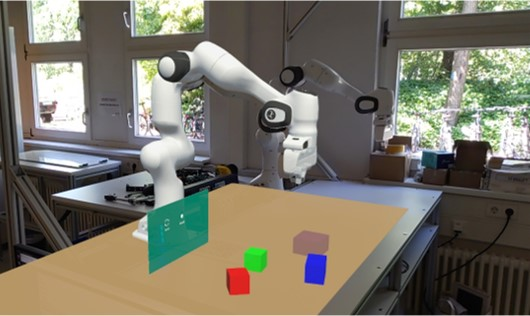
\includegraphics[width=\linewidth]{img/AR/Virtual_Robot.jpg}}
        %\captionsetup{margin={2mm,0mm}}
        %\caption{}
        \label{subfig:Virtual_Robot}
    \end{subfigure}
   % \hfill
   % \hspace{0.02cm}
    \begin{subfigure}{0.2\textwidth}
        \raisebox{0.315cm}{
        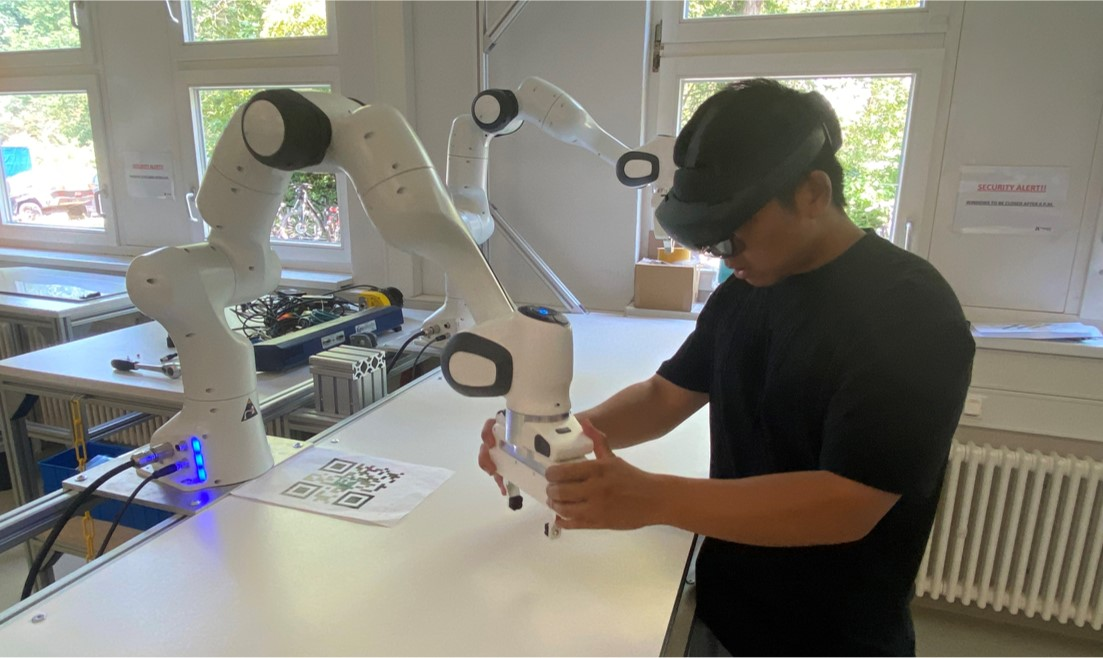
\includegraphics[width=\linewidth]{img/AR/Creating_Demonstrations.jpg}}
        %\captionsetup{margin={2mm,0mm}}
        %\caption{}
        \label{subfig:Creating_Demonstrations}
    \end{subfigure}
   % \hfill
   % \hspace{0.02cm}
    \begin{subfigure}{0.2\textwidth}
        \raisebox{0.315cm}{
        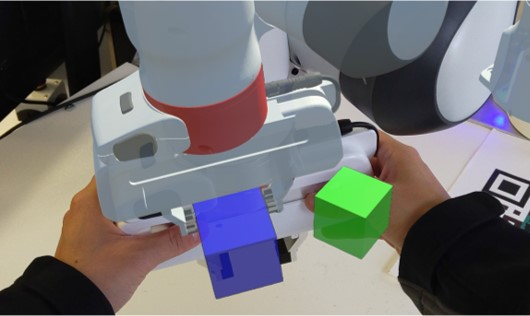
\includegraphics[width=\linewidth]{img/AR/User_View.jpg}}
        %\captionsetup{margin={2mm,0mm}}
        %\caption{}
        \label{subfig:User_View}
    \end{subfigure}
   % \hfill
   % \hspace{0.02cm}
    \begin{subfigure}{0.32\textwidth}
        \raisebox{0.075cm}{
        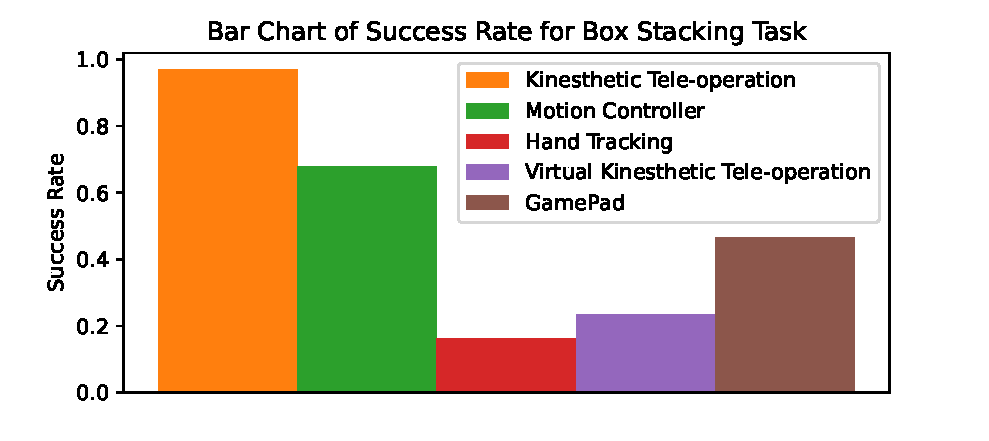
\includegraphics[width=\linewidth]{img/AR/success_rate.pdf}        
        }
        \label{subfig:objective_metric_Success_all}
    \end{subfigure}
%    \hfill  
    % \hspace*{\fill}%    
    \vspace{-0.5cm}
    \caption{\small{\textit{The AR-enhanced data collecting platform from our prior work \cite{jiang2023user}. (left) The virtual robot and objects. (mid-left) Utilizing HoloLens 2 to create human demonstrations. (mid-right) Perspective from the AR user. %(right) Comparison for five interfaces, showing our interface "kinesthetic tele-operation" depicting the highest success rates.
    (right) Our interface "kinesthetic tele-operation" depicts the highest success rates compared to baselines.}}}
    \label{fig:AR_image}
  %  \vspace{0.3cm}
\end{figure}